\documentclass{article}
\usepackage[latin1]{inputenc}
\usepackage[ngerman]{babel}
\usepackage{graphicx}
\usepackage{enumitem}
\usepackage{multirow}
\usepackage{threeparttable}
\usepackage{lscape}

\begin{document}

\title{Automatisierung der WSUS Auswertung
\\ Ein Projekt mit PHP\textbackslash MSSQL}
\author{Gennaro Piano}
\date{\today}

\maketitle

\begin{figure}[htbp]
		\centering
	
\includegraphics[width=10cm]{wsus.jpg}
		\label{fig:logo}
\end{figure}

\newpage
\tableofcontents
\newpage
\section{Einleitung}
\subsection{Ausgangslage}
Wir bieten unseren Kunden die M�glichkeit die Windows Updates �ber unserem WSUS Server herunterzuladen. Durch dieses Angebot muss sich der Kunde nicht mehr �ber fehlerhaften Updates k�mmern, da wir die Updates zuerst in einer Testumgebung testen und diese danach freigeben. Um die Updateverwaltung einfach zu halten wurden auf dem WSUS Server Produktklassen erstellt. Computer und Server von Kunden die unser Angebot nutzen m�chten, werden den entsprechenden Produktklassen zugeteilt. Updates die freigegeben sind werden wiederum den entsprechenden Produktklassen zugeteilt und somit auf den Ger�ten der Kunden installiert. Dieses System ist gut durchdacht, jedoch ist es sehr kompliziert diese Daten auszuwerten. \newline \newline
Um die Daten auszuwerten werden jedes Quartal alle freigegebenen Updates manuell in einer Excel Datei aufgenommen. Jedes Update wird danach in die entsprechende Produktklasse kopiert. Auf einem weiterem Excel Blatt wird ausgewertet, welcher Benutzer welche Produktklassen ben�tigt. Dieser Prozess ist sehr zeitintensiv und kostet pro Quartal circa eins bis zwei Arbeitstage.
\subsection{Ziel der Arbeit}
Um den Aufwand zu k�rzen soll der Ablauf des Prozesses so weit wie m�glich automatisiert werden. Dies soll mit PHP und einem MS SQL Server realisiert werden. Im ersten Schritt soll die Verbindung zwischen den Updates und den Produktklassen programmiert werden. Als zweiter Schritt werden die Kunden hinzugef�gt und die Auswertung automatisiert. Diese Arbeit befasst sich mit dem ersten Schritt des Projekts.
\newpage
\section{Requierements}
\subsection{Einleitung}
\textbf{Zweck} \newline
Dieser Teil des Dokuments befasst sich mit den Anforderungen, des Projekts. Diese Anforderungen werden mit dem Auftraggeber angeschaut. Erst wenn die Anforderungen vom Auftraggeber best�tigt worden sind und nach seiner Meinung alles abgedeckt ist, wird das Projekt fortgef�hrt.
\newline
\newline
\textbf{Systemumfang} \newline
Das System wird f�r den internen Gebrauch entwickelt und soll von aussen nicht zug�nglich sein. Somit besteht keine Gefahr, die Applikation vor unerlaubten Zugriff zu sch�tzen, da dies die Firewall handhabt. 
\newline
\newline
\textbf{Auftraggeber} \newline
Der Auftraggeber dieses Projekts ist zugleich der interne technische Leiter der Firma. Somit wird das Projekt als internes Projekt gehandhabt. Der technische Leiter ist kein Programmierer und stellt deswegen keine technische Anforderungen an das Projekt. Der technische Leiter wird f�r dieses Projekt als Kunde angesehen.\newline \newline
\subsection{Allgemeine �bersicht}
\textbf{Systemumfeld} \newline
Diese Applikation ben�tigt einen Webserver und eine Schnittstelle zu einer Microsoft SQL Datenbank. Der WSUS Server geh�rt auch zum Systemumfeld, jedoch ist die Verbindung zwischen dem WSUS Server und der Applikation nur abstrakt, da die entnommenen Informationen aus dem WSUS Server manuell in der Applikation aufgenommen werden.
\begin{figure}[htbp]
		\centering
	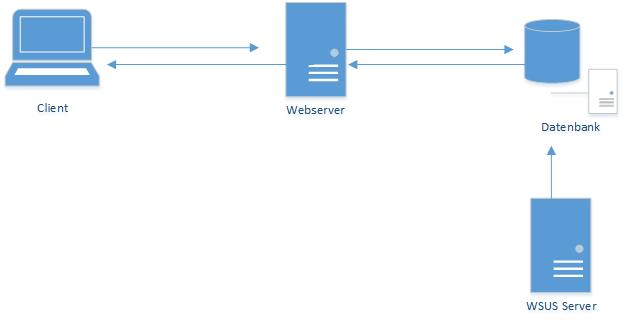
\includegraphics[width=10cm]{C:/inetpub/wwwroot/auswertung/doc/img/Systemumfeld.jpg}
		\label{fig:Systemumfeld}
\end{figure}
\newpage
\parindent0pt \textbf{Architekturbeschreibung} \newline
Die PHP Applikation wird auf dem schon vorhandenen Webserver implementiert. Es handelt sich um einen IIS, dies ist der Webserver von Microsoft. Der IIS unterst�tzt von sich aus kein PHP. Somit muss der PHP Interpreter nachger�stet werden. Der PHP Interpreter wird mit dem integrierten Webplattform Installer installiert. F�r die Datenbankanbindung wird ebenfalls der vorhandene SQL Server benutzt. Auf diesem Server wird eine neue Datenbank und ein neuer Datenbankbenutzer erstellt. Der neue Benutzer wird nur auf diese Datenbank Zugriff haben, zugleich wird er der einzige Benutzer sein, der auf die neue Datenbank Zugriff hat. Der Webserver und der SQL Server befinden sich physikalisch auf dem gleichen Server, somit ist hardwarem�ssig nur ein Server von den Ver�nderungen betroffen. Der PHP Interpreter ben�tigt eine Schnittstelle um auf die Datenbank zu lesen und zu schreiben, die Schnittstelle zwischen PHP und einem Microsoft SQL Server wird nicht automatisch installiert und muss somit manuell nachinstalliert werden.
\newline
\newline
\textbf{Systemfunktionalit�t} \newline
Das Use Case Diagramm soll die Funktionalit�t des Systems aufzeigen.
\begin{figure}[htbp]
		\centering
	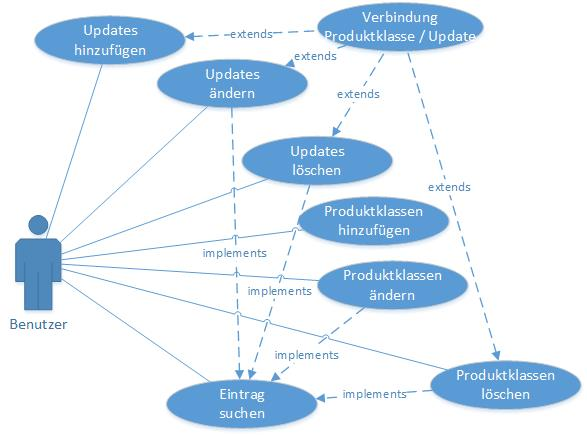
\includegraphics[width=14.5cm]{C:/inetpub/wwwroot/auswertung/doc/img/Use_Case.jpg}
		\label{fig:UseCaseDiagramm}
\end{figure}
\newpage
\parindent0pt \textbf{Nutzer und Zielgruppen} \newline
Der Hauptnutzer ist zugleich der Auftraggeber dieses Projekts. Neben dem Auftraggeber wird die Webapplikation auch von seinem Stellvertreter benutzt werden, dies wird jedoch sehr selten der Fall sein. Der Zugriff auf die Webapplikation wird f�r alle Benutzer des Unternehmens m�glich sein, dies ist bei der momentanen Excel Datei auch der Fall.
\newline
\newline
\textbf{Annahmen} \newline
Der zweite Teil des Projekts wird wie oben bereits erw�hnt erst sp�ter entwickelt. In dieser Dokumentation wird auf den zweiten Teil des Projekts bewusst nicht eingegangen, da dies ansonsten den Umfang dieses Dokuments sprengen w�rde.
\subsection{Anforderungen}

\subsection{Analyse der Anforderungen}
\end{document}
